\documentclass[11pt,a4paper,leqno,titlepage,twoside]{book}

\usepackage{mystylearticle}
\usepackage{balance}
\usepackage{multicol} 
\usepackage{nonfloat}
\usepackage{enumitem}
\usepackage{wallpaper}
\usepackage{sectsty}
\usepackage[utf8]{inputenc} %para los acentos

%%%%%% Fuente por defecto %%%%%%%%%%
\renewcommand{\familydefault}{\sfdefault}


%%%%%% Figuras especiales %%%%%%%%%%
\newcommand\myfigure[1]{%
\bigskip\noindent\begin{minipage}{\linewidth}%{0.9\columnwidth}
\centering%
#1%
%figure,caption, and label go here
\end{minipage}\medskip}

%%%%%% Nombres %%%%%%%%%%
\renewcommand{\contentsname}{Contenidos}
\renewcommand{\chaptername}{Cap\'\i tulo}
\renewcommand{\bibname}{Bibliograf\'\i a}
\renewcommand{\figurename}{Figura}

%%%%%% Página en blanco %%%%%%%%%%

\def\blankpage{%
      \clearpage%
      \thispagestyle{empty}%
      \addtocounter{page}{-1}%
      \null%
      \clearpage}


%%%%%% Colores del tema %%%%%%%%%%
\definecolor{oyellow}{rgb}{1,0.835294117647059,0.133333333333333}
\definecolor{oblue}{rgb}{0.0352941176470588,0.450980392156863,0.541176470588235}
\definecolor{ogreen1}{rgb}{0.0196078431372549,0.650980392156863,0.576470588235294}
\definecolor{ogreen2}{rgb}{0.0588235294117647,0.737254901960784,0.568627450980392}
\definecolor{ored}{rgb}{0.929411764705882,0.258823529411765,0.215686274509804}

%%%%%% Secciones con color %%%%%%%%%%
\chapterfont{\color{oblue}}
\sectionfont{\color{oblue}}
\subsectionfont{\color{ogreen1}}
\subsubsectionfont{\color{ogreen2}}


%%%%%% Referencias con color %%%%%%%%%%
\hypersetup{colorlinks=true,
			linkcolor = oblue,
            urlcolor  = oblue,
            citecolor = oblue,
            anchorcolor = oblue}

%%%%%% Gráficos %%%%%%%%%%			
% \graphicspath{{../pdf/}{C:/DATOS/MBIT/Memoria/graphs/}}
\graphicspath{{../pdf/}{C:/DATOS/MBIT/Proyecto/MBITProject_Data4all/Memoria/graphs/}}

%%%%%% Headers and footers %%%%%%%%%%
\pagestyle{fancy}
\renewcommand{\sectionmark}[1]{\markright{\thesection\ #1}}
\fancyhf{}
% \fancyhead[LO]{\tt Versi\'on preliminar \today}
% \fancyhead[RE]{\tt Versi\'on preliminar \today}

\newcommand\PageBoxODD{
	\setlength{\fboxrule}{0cm}
	\fcolorbox{oyellow}{oyellow}{\begin{minipage}[t][0.75cm][c]{\textwidth}{\qquad\bf OCTOPUS} DATA INSIGHTS \hfill \thepage\qquad$ $\end{minipage}}}
	
\newcommand\PageBoxEVEN{
	\setlength{\fboxrule}{0cm}
	\fcolorbox{oyellow}{oyellow}{\begin{minipage}[t][0.75cm][c]{\textwidth}{\qquad\thepage\hfill\bf OCTOPUS} DATA INSIGHTS\qquad$ $\end{minipage}}}

\fancyfoot[CE]{\PageBoxEVEN}
\fancyfoot[CO]{\PageBoxODD}

\renewcommand{\headrulewidth}{0pt}
\renewcommand{\footrulewidth}{0pt}


\fancypagestyle{plain}{%
  \fancyhf{}%
  \renewcommand{\headrulewidth}{0pt}
  \fancyfoot[CE]{\PageBoxEVEN}
  \fancyfoot[CO]{\PageBoxODD}
}




% %%%%%%%%%%%%%%%%%%%%%%%%%%%%%%%% BEGIN DOCUMENT %%%%%%%%%%%%%%%%%%%%%%%%%%%%%%%%%%%%%%

\begin{document}

%Title  page

\begin {titlepage}
% Picture with pgf
\begin{pgfpicture}{0cm}{0cm}{\textwidth}{\textheight}
% Background picture
\pgfputat{\pgfxy(-12,-4)}{\pgfbox[center,center]{\begin{picture}(0,0)(0,0)\resizebox{40cm}{30cm}
{
\includegraphics{portada.jpg}}\end{picture}}}
% Title and authors
\pgfputat{\pgfxy(0,5)}{\pgfbox[left,center]{\Huge\textbf{AN\'ALISIS DE REDES SOCIALES}}}
\pgfputat{\pgfxy(0,4)}{\pgfbox[left,center]{\Huge\textbf{PARA RECURSOS HUMANOS}}}
\pgfputat{\pgfxy(0,2)}{\pgfbox[left,center]{\textbf{Fabio Inui\qquad Teresa Mart\'\i nez \qquad Javier Quintana \qquad Silvia Santos }}}

% PARA VERSIONES PRELIMINARES
\pgfputat{\pgfxy(0,1)}{\pgfbox[left,center]{\textbf{Versión preliminar \today}}}

\end{pgfpicture}
\end {titlepage}

%%% End Title page

% Ojo, la p\'agina en blanco detr\'as de la portada
\blankpage

%%%% Dedicatoria

\pagestyle{empty}
\vspace*{4cm}
\hfill\begin{minipage}[t][0.75cm][c]{0.5\textwidth}\flushright
Dedicamos esta memoria a nuestras familias, sin cuya paciencia sin l\'imites, no hubiera sido posible su elaboraci\'on.
Agradecemos a nuestros profesores ({\bf a unos m\'as que a otros}) su dedicaci\'on y ayuda.
\end{minipage}
\addtocounter{page}{-2}

%%%% Dedicatoria

% Ojo, la p\'agina en blanco detr\'as de la dedicatoria
\blankpage

\pagestyle{fancy}



%Table of contents, the document begins in a new page.

\tableofcontents


\newpage

\chapter*{Resumen ejecutivo}
\addcontentsline{toc}{chapter}{Resumen ejecutivo}


\chapter*{Executive summary}
\addcontentsline{toc}{chapter}{Executive summary}



\chapter{Planteamiento del proyecto}

En este cap\'\i tulo vamos a describir las ideas y contexto en el que vamos a desarrollar el contenido del proyecto.

\section{Descripci\'on}
Cuando un departamento de Recursos Humanos o una empresa de reclutamiento se enfrenta a una petici\'on para
cubrir un puesto vacante o de nueva creaci\'on, el proceso suele llevarse a cabo en diversas fases, que 
podr\'\i amos describir del siguiente modo \cite{proceso_seleccion1}:
\begin{enumerate}
\item {\bf Preselección}: etapa inicial en la que se detectan candidatos adecuados para el perfil buscado, bien recurriendo a 
anuncios en portales especializados, bien con b\'usquedas personalizadas de perfiles. En esta etapa se elabora una lista 
de candidatos que pasar\'an a las siguientes fases del proceso, descartando aquellos cuyas competencias no sean las adecuadas
para el puesto. 
\item {\bf Entrevista inicial}: en esta etapa los candidatos seleccionados en la etapa anterior son contactados para  
conseguir ampliar la informaci\'on de la que se dispone sobre ellos  (por ejemplo sobre las aptitudes
particulares y experiencias previas consignadas en el CV), y verificar el inter\'es y compromiso del candidato
con respecto a la oferta.
\item {\bf Informe}: tras la entrevista inicial, se seleccionan los mejores candidatos para el puesto, y se realiza un informe
donde se consignan los datos originales (el CV, por ejemplo) y los datos a\~nadidos en el curso de la entrevista inicial.
\item {\bf Presentaci\'on de candidatos}: el empleador recibe el informe elaborado en el punto anterior, y selecciona aquellos
que mejor se ajusten a sus necesidades, muy habitualmente realizando nuevas entrevistas con ellos.
\item {\bf Decisi\'on}: es el momento en que se elige el candidato al que se se le va a ofrecer el puesto, etapa en la 
que puede complementarse la informaci\'on recogida hasta el momento con referencias recabadas de anteriores empleadores.
\item {\bf Oferta}: etapa en la que la empresa presenta al candidato la oferta en firme, habitualmente por escrito, consignando 
la voluntad de la empresa de incorporar al candidato y los detalles econ\'omicos. 
\item: {\bf Seguimiento}:  para comprobar que una vez incorporado a la empresa, tanto empleado como empleador est\'an conformes con
el resultado del proceso.
\end{enumerate}

Tradicionalmente, el comienzo de este proceso, la detecci\'on de candidatos, se realizaba en numerosas ocasiones 
a trav\'es de anuncios en prensa,
bases de datos de candidatos construidas a lo largo del tiempo, y la explotaci\'on de la red de contactos personales del entorno 
del empleador. Hoy por hoy, estos m\'etodos tradicionales han sido complementados, y algunos dir\'\i an que pr\'acticamente
suplantados, por m\'etodos que explotan la informaci\'on contenida en la web. 

Los t\'ecnicos de selecci\'on se enfrentan a un mundo muy diverso donde tanto la difusi\'on de los 
posibles puestos como la informaci\'on sobre los candidatos para los mismos est\'a diseminada en numerosos
formatos, teniendo un papel preponderante diversas plataformas o portales web (InfoJobs, Monster, etc.)
y redes sociales en general (LinkedIn, Twitter, Facebook, Instagram, etc.). Desde el punto de vista del t\'ecnico de selecci\'on, las
primeras contienen mucha informaci\'on sobre las aptitudes de los posibles candidatos, sus conocimientos, formaci\'on y 
experiencia, ya que son portales donde los propios usuarios consignan sus curricula vitae, y tambi\'en sobre su situaci\'on laboral
actual y expectativas. En el segundo grupo de fuentes, las redes sociales, hay algunas que tienen el car\'acter espec\'\i fico 
de las primeras (LinkedIn es el ejemplo m\'as claro), y hay otras en las que se consigna informaci\'on diversa, llam\'emoslas de 
prop\'osito general, tal vez en mayor medida personal que profesional.

El objetivo de nuestro proyecto es complementar el 
trabajo habitual de un departamento de Recursos Humanos o de un seleccionador de personal en
los portales y redes sociales dedicados al mundo laboral, con informaci\'on laboral extra\'\i da 
de fuentes menos est\'andar, como son las redes sociales de prop\'osito general. 
Estas redes son a menudo aprovechadas por los usuarios para difundir mensajes relacionados con su actividad
laboral, y una descripción de su actividad en las redes es relevante desde el punto de vista 
de un reclutador, en la medida que da informaci\'on del compromiso de la persona con su actividad, su valoración por
parte de otros usuarios, su proactividad, etc.

En este trabajo hemos elegido la red social Twitter por diversos motivos: es una de las redes más dinámicas,
con millones de usuarios activos en todo el mundo, fácil de usar, rápida y divertida. 

\myfigure{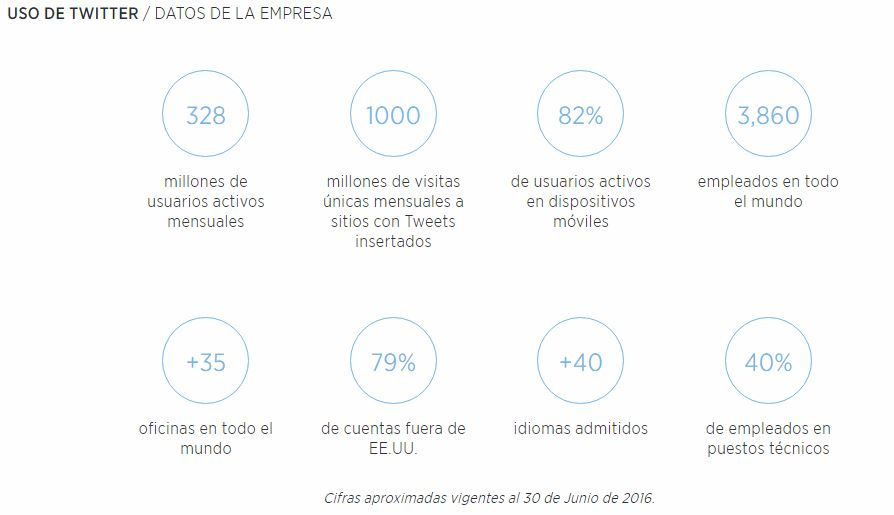
\includegraphics[width=0.6\textwidth]{twitter_uso_y_empresa}%
\figcaption{Twitter: uso y datos de la empresa, \url{https://about.twitter.com/es/company}.}
\label{fig:twitter_uso_y_empresa} }


Esta red da cabida a relaciones diversas, entre usuarios de variada índole. Dado que muchos de los usuarios 
twitean información relacionada con su ocupación laboral, es natural esperar que en Twitter 
se formen comunidades de individuos que comparten interés en diferentes aspectos de dicho ámbito.
Nuestro propósito es definir e implementar un proceso que permita agregar información referente a 
esas comunidades extraer de Twitter aquellos tuits 
cuyo contenido sea 

Es decir, tras el proceso habitual de:

1. Apertura de la vacante
2. Recepci\'on de CVs
3. Descarte y Selecci\'on previa de CV

…. aqu\'{\i} en este punto de la fase es donde creo que puede aportar informaci\'on adicional que le sirva para hacer un 
pre-ranking de candidatos…

4. Entrevistas
5. “Short-list” y valoraci\'on final

-… y creo que en el punto final tambi\'en puede ser un atributo determinante si en el proceso dudan entre dos candidatos 
finales, por ejemplo.

Y para tratar de plasmar de alguna forma a que me estoy refiriendo y como podemos enfocarlo, trato de explicarlo con un ejemplo.

Imaginemos que buscamos el mejor “data scientist” en Madrid y que ya tienen dos candidatos que les encajan y que han estado bien 
en las entrevistas. ¿c\'omo decidir?…pues con informaci\'on complementaria de como est\'an valorados en su propio sector.

Pongamos por caso que nuestros dos candidatos son:

 

Nota. Un problema a resolver es que no todo el mundo pone su perfil de twitter en la informaci\'on de linkedin que es la fuente 
principal de informaci\'on en un proceso de selecci\'on y de alguna forma hay que poder cruzar esos datos. En este ejemplo he 
tomado dos casos que si incluyen dicha informaci\'on.

El primer paso es disponer de sus perfiles en twitter:

 		 

Y a partir de aqu\'{\i} hacer valoraciones que nos permitan crear una especie de ranking:

•	Trabajan en lo que dicen?
•	Siguen a perfiles del sector?
•	Son seguidos por perfiles del sector?
•	Hacen comentarios profesionales o mas bien personales?
•	C\'omo de valorados est\'an estos comentarios?
•	…






Por ejemplo, y sin ser una comparativa ni exhaustiva ni exacta:

Sixto Villalba
Nuestro primer candidato parece tener un perfil m\'as amplio y heterog\'eneo, y adem\'as, por el enlace que tiene a su 
“wordpress” podemos comprobar que est\'a m\'as centrado en “SEO/SEM y Marketing Digital” que en “Big Data” (hay forma de 
poder incluir esto en el modelo?..habr\'a que verlo)
https://sixtoseovb.wordpress.com

El tipo de tuits no se limitan solo al trabajo y sus seguidores tambi\'en son heterog\'eneos…, aunque su actividad es m\'as intensa..


Diego J. Bodas
Perfil m\'as reducido y menos intenso que el otro candidato, pero mucho m\'as centrado en el “Big Data” (al menos en un primer vistazo jj)..

No se si con esto me explico….o a\'un os lio m\'as…jejejejeje

Y tambi\'en por lo que he podido ir leyendo sobre Twitter, cosas que en principio creo que se pueden obtener:

•	Obtener tuits generales, trending topics, tuits que contienen un hastag o una palabra en concreto
•	Una vez obtenido se puede “limpiar” para quedarnos con lo que nos interese. Una de las cuestiones interesantes es por ejemplo la “geolocalizaci\'on” de los tweets (no se de momento para que pero puede ser \'util…)
•	What entities are in a user's tweets?
What are the most frequently occurring entities that appear in a user's tweets?
Who does a given user retweet the most often?
How many of a user's tweets contain hashtags?
How many of a user's tweets get retweeted?
How many of a user's tweets contain at least one entity?
•	Here, I will show you two cases:
•	1) What are the hashtags utilized by different users?
•	2) Who retweets whom?
•	Quien retuitea y sigue a quien y completarlo con
•	Analisis de sentimiento
(en este enlace se explica….

http://www.slideshare.net/mcjenkins/how-sentiment-analysis-works





\section{Contexto de negocio}
Lo que hay hecho y lo que no.
\section{Objetivos}
Lo que queremos conseguir, qué significa que lo hayamos conseguido.
\section{Hip\'otesis y limitaciones}
Aquí todo lo que asumamos al plantear el proyecto, y hasta dónde puede llegar. Límites del uso de la información
de las redes sociales, límites del proceso en sí (ventana temporal, no detección de todos los candidatos, etc.).
\subsection{La Ley Orgánica 15/1999, de 13 de diciembre, de Protección de Datos
de Carácter Personal}
Cómo nos afecta. Malamente.

\chapter{Planificación del proyecto}
\section{Equipo}
El equipo de Octopus Data Insights está formado por cuatro personas, con perfiles multidisciplinares y complementarios:
\begin{itemize}
\item Fabio Inui: 
\item Teresa Martínez: matemática, con diez años de experiencia en investigación y docencia a nivel universitario,
ocho en construcción de modelos de valoración de derivados en empresa financiera de primer nivel, y cuatro de
gestión de fondos en una de las principales gestoras españolas.
\item Javier Quintana: 
\item Silvia Santos: 
\end{itemize}
\section{Desarrollo temporal}

\chapter{Infraestructura}
En esta sección describiremos la infraestructura que hemos construido para el desarrollo del proyecto.
\section{Repositorio GIT}
El código del proyecto, así como las presentaciones y memoria de este proyecto, está almacenado en el 
repositorio \url{https://github.com/MaiteMartinez/MBITProject_Data4all}

\myfigure{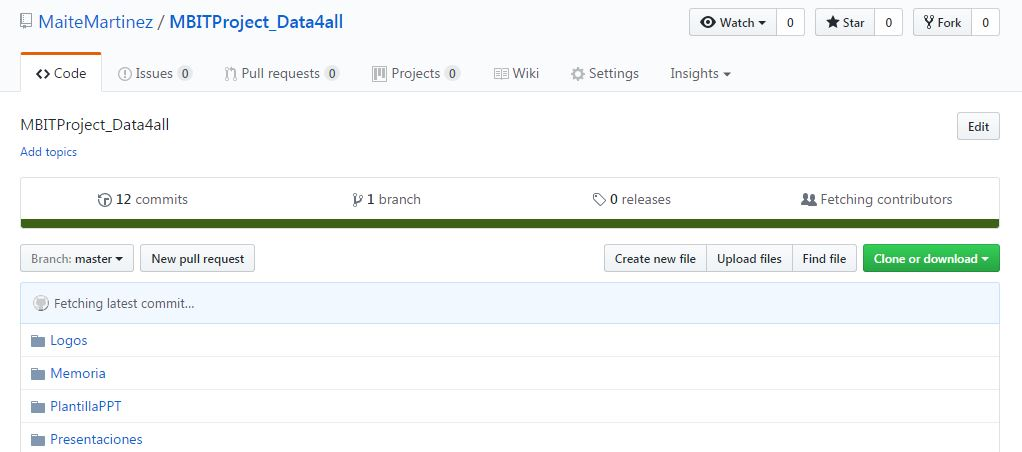
\includegraphics[width=0.6\textwidth]{repositorio_git1}%
\figcaption{Repositorio del código del proyecto.}
\label{fig:repositorio_git1} }

\section{Infraestructura para la obtención de datos}
\section{Desarrollo en la nube}

\chapter{Tratamiento inicial de los datos}
\section{Descripci\'on de los datos}
Estructura general de los tuits y campos necesarios para nuestro objetivo. 
\section{Obtenci\'on de los datos}
C\'omo hemos hecho para bajarlos, par\'ametros de la b\'usqueda de twits.
\section{Almacenamiento}
\section{Limpieza de los datos}

\chapter{Preparaci\'on de los datos}
\section{Extracci\'on de la informaci\'on relevante}
\section{Almacenamiento}

\chapter{Modelado de los datos}
\section{Principales hip\'otesis}
\section{Algoritmos}
\section{Almacenamiento}

\chapter{Visualizaci\'on de los resultados}
\section{Herramientas}
\section{Acceso web}

\chapter{\'Areas de mejora}



% \myfigure{\includegraphics[width=.9\columnwidth]{Master_bond_avg_spr_table}%
% \figcaption{Master Bond: ``mid-market" g-spreads by rating.}
% \label{fig:Master_bond_avg_spr_table} }




\begin{thebibliography}{3}
\addcontentsline{toc}{chapter}{Bibliograf\'\i a}

\bibitem{proceso_seleccion1} 
Mar\'\i a Gloria Casta\~no collado, Gerardo de la Merced L\'opez Montalvo, Jos\'e Mar\'\i a Prieto Zamora,
\textit{Gu\'\i a t\'ecnica y de buenas pr\'acticas en reclutamiento y selecci\'on de personal (R\& S)}.
Documento aprobado por la Junta de Gobierno del Colegio Oficial de Psicólogos de Madrid, Febrero de 2011.
\url{http://www.copmadrid.org/webcopm/recursos/guiatecnicabuenaspracticas.pdf}

\bibitem{proceso_seleccion2} 
\textit{Selecci\'on de personal para no especialistas}.
Andaluc\'\i a Emprende, Fundaci\'on P\'ublica Andaluza. Consejer\'\i a de Econom\'\i a y Conocimiento.
\url{https://www.andaluciaemprende.es/wp-content/uploads/2015/02/guia\-seleccion-personal.pdf}

\bibitem{lopd1} 
\textit{Ley Orgánica 15/1999, de 13 de diciembre, de Protección de Datos
de Carácter Personal}.
Jefatura del Estado BOE núm. 298, de 14 de diciembre de 1999
Referencia: BOE-A-1999-23750
\url{http://www.agpd.es/portalwebAGPD/canaldocumentacion/legislacion/estatal/common/pdfs/2014/Ley_Organica_15-1999_de_13_de_diciembre_de_Proteccion_de_Datos_Consolidado.pdf}

\bibitem{tesis_mariluz} 
María Luz Congosto Martínez,
\textit{Caracterización de usuarios y propagación de mensajes en Twitter en el entorno de temas sociales}.
Tesis doctoral.

\bibitem{twitter_wikipedia} 
``Twitter". Wikipedia. \url{https://es.wikipedia.org/wiki/Twitter}.

\bibitem{kumar_et_al}Shamanth Kumar, Fred Morstatter, Huan Liu. 
{\em  Twitter Data Analytics}. Springer (2013).

\bibitem{twitter_dev_web} Twitter Developer Documentation{\url https://dev.twitter.com/}

\bibitem{nltk_book}Steven Bird, Ewan Klein, Edward Loper. {\em Natural Language Processing with Python: 
Analyzing Text with the Natural Language Toolkit}. O'Reilly (2009). \url{http://www.nltk.org/book/}

\bibitem{zissman-berkling} Marc A. Zissman, Kay M.Berkling. Automatic language identification. {\em Speech Communication}, 
Volume 35, Issues 1–2, August 2001, Pg. 115-124.

\bibitem{almeida_estevez_piad} Y. Almeida-Cruz, S. Estévez-Velarde, A.  Piad-Morffis. Detección de Idioma en Twitter.
{\em GECONTEC: Revista Internacional de Gestión del Conocimiento y la Tecnología}, Vol.2 (3), 2014.
\url{https://www.upo.es/revistas/index.php/gecontec/article/view/1081/pdf_11}

\bibitem{langid} Marco Lui, Timothy Baldwin. {\tt langid.py}: An Off-the-shelf Language Identification Tool.
{\em Proceedings of the ACL 2012 System Demonstrations}, pg. 25--30, 2012.
\url{http://www.aclweb.org/anthology/P12-3005}

\bibitem{langid2} Marco Lui, Timothy Baldwin. Accurate Language Identification of Twitter Messages. 
{\em Proceedings of the 5th Workshop on Language Analysis for Social Media (LASM) @ EACL 2014}, pg. 17-–25,
(2014). \url{http://www.aclweb.org/anthology/W14-1303}

\bibitem{equilid} David Jurgens, Yulia Tsvetkov, Dan Jurafsky. Incorporating Dialectal Variability
for Socially Equitable Language Identification. 
{\em Proceedings of the 55th Annual Meeting of the Association for Computational Linguistics (Short Papers)}, 
pg. 51-–57, (2017). \url{https://doi.org/10.18653/v1/P17-2009}

\bibitem{libro_rrhh} Tobias M. Scholz. {\em Big Data in Organizations and the Role of
Human Resource Management}, Peter Lang Academic Research, Series: Personalmanagement und
Organisation, Vol. 5 (2017).

\bibitem{user_class1}Marco Pennacchiotti, Ana-Maria Popescu. A Machine Learning Approach to Twitter User 
Classification, AAAI Publications, Fifth International AAAI Conference on Weblogs and Social Media (2011).
\url{https://webpages.uncc.edu/anraja/courses/SMS/SMSBib/2886-14198-1-PB.pdf }

\bibitem{user_class2} Anjie Fang, Iadh Ounis, Philip Habel, Craig Macdonald, Nut Limsopatham.
Topic-centric Classification of Twitter User’s Political Orientation. Proceedings of the 
6th Symposium on Future Directions in Information Access (2015).
\url{http://www.dcs.gla.ac.uk/~anjie/papers/fang2015fdia.pdf }

\bibitem{user_class3} Tomoya Noro, Atsushi Mizuoka, Takehiro Tokuda. 
Towards Finding Good Twitter Users to Follow Based on User Classification.
Proceedings of The 24th International Conference on Information Modelling and Knowledge 
Bases (2014). \url{https://www.researchgate.net/publication/269994032_Towards_Finding_Good_Twitter_Users_to_Follow_Based_on_User_Classification }

\bibitem{user_class4} Zi Chu, Steven Gianvecchio, Haining Wang, Sushil Jajodia. 
Detecting Automation of Twitter Accounts: Are You a Human, Bot, or Cyborg?
IEEE Transactions on Dependable and Secure Computing, Vol. 9 (2012).
\url{http://www.cs.wm.edu/\~ hnw/paper/tdsc12b.pdf }.

\bibitem{user_class5} Yan L., Ma Q., Yoshikawa M.. Classifying Twitter Users Based on User Profile and Followers Distribution. En: Decker H., Lhotská L., Link S., Basl J., Tjoa A.M. (eds) Database and Expert Systems Applications. DEXA 2013. Lecture Notes in Computer Science, vol 8055. Springer (2013).
\url{https://link.springer.com/chapter/10.1007/978-3-642-40285-2_34 }.

\bibitem{talent_an} Jasmit Kaur, Alexis A. Fink. Trends and Practices in Talent
Analytics. SHRM-SIOP Science of HR White Paper Series (2017).
\url{http://www.siop.org/SIOP-SHRM/2017%2010_SHRM-SIOP%20Talent%20Analytics.pdf }

\bibitem{notas_fernando} Fernando Pérez García. Teoría de Grafos. Notas de las clases
impartidas en el Máster en Data Science, MBIT, convocatoria Marzo 2017.

\bibitem{bonacich} Phillip Bonacich, Paulette Lloyd. 
Eigenvector-like measures of centrality for asymmetric relations.
{\em Social Networks}, 23, pg. 191–201 (2001).
\url{http://citeseerx.ist.psu.edu/viewdoc/download?doi=10.1.1.226.2113&rep=rep1&type=pdf }

\bibitem{bonacich2} Phillip Bonacich. A Family of Measures. {\em American Journal 
of Sociology}, Vol. 92, No. 5, pg 1170-1182 (1987). 
\url{http://www.leonidzhukov.net/hse/2014/socialnetworks/papers/Bonacich-Centrality.pdf }.

\bibitem{kleinberg}Jon M. Kleinberg. Authoritative sources in a hyperlinked environment.
{\em Journal of the ACM (JACM)}, Vol. 46, Issue 5 (1999).
\url{http://www.cs.ucr.edu/~vagelis/classes/CS172/publications/kleinberg98authoritative.pdf } 


\bibitem{user_class} Lalindra De Silva, Ellen Riloff. User Type Classification of Tweets with Implications 
for Event Recognition. Proceedings of the Joint Workshop on Social Dynamics and Personal Attributes 
in Social Media (2014).
\url{https://www.cs.utah.edu/~riloff/pdfs/DeSilva-SMWorkshop-ACL14.pdf }

\bibitem{fdez} Pablo Fernández Gallardo. Google’s secret and Linear Algebra,
 EMS Newsletter, vol. 63, pg. 10-15 (2007)

\bibitem{notas_alvaro} Álvaro Romero. Sistemas de Recomendación. Notas de las clases
impartidas en el Máster en Data Science, MBIT, convocatoria Marzo 2017.

\bibitem{notas_antonio} Antonio LaTorre. Aprendizaje supervisado. Notas de las clases
impartidas en el Máster en Data Science, MBIT, convocatoria Marzo 2017.
\end{thebibliography}


\newpage

%%%%% añade una pagina en blanco si el numero final de la pagina es impar

\cleardoublepage

%%%%%%%%%%%%%%las dos paginas finales, tipeset with latex y contraportada

\clearpage%
\thispagestyle{empty}%
\vspace*{\fill}
\begin{center}
    \sf Documento producido con \LaTeX.
\end{center}
\vspace*{\fill}
\addtocounter{page}{-1}%
\null%
\clearpage

\pagestyle{empty}
% Picture with pgf
\begin{pgfpicture}{0cm}{0cm}{\textwidth}{\textheight}

% Background picture
\pgfputat{\pgfxy(-12,-4)}{\pgfbox[center,center]{\begin{picture}(0,0)(0,0)\resizebox{40cm}{30cm}
{
\includegraphics{contraportada.jpg}}\end{picture}}}
\end{pgfpicture}

\end{document}
	






